\documentclass[12pt, a4paper, openany]{report}

\usepackage[left=3cm,top=3cm, bottom=3cm, right=4cm]{geometry}

\usepackage{secdot} % Dots in Section Numbers
\usepackage[utf8]{inputenc}
\usepackage[ngerman]{babel}
\usepackage{graphicx}
\graphicspath{ {images/} }

\usepackage{fancyhdr}
\usepackage{todonotes}
\usepackage{hyperref}

\usepackage{titlesec}
\titleformat{\chapter}[hang]{\Huge\bfseries}{}{0pt}{\Huge\bfseries}
\newcommand\frontmatter{ \cleardoublepage \pagenumbering{roman}}
\newcommand\mainmatter{ \cleardoublepage \pagenumbering{arabic}}
\newcommand\backmatter{ \if@openright \cleardoublepage \else \clearpage \fi }

\usepackage[autostyle]{csquotes}
\usepackage[
    backend=biber,
    style=alphabetic,
    sortlocale=de_DE,
    natbib=true,
    url=false,
    doi=true,
    eprint=false
    ]{biblatex}
\addbibresource{literatur.bib}

\usepackage{xparse}
\DeclareDocumentCommand \footATCite{ O{} o m } {%
  \IfNoValueTF {#2} {\footnote{#1 \citeauthor{#3}, \emph{\citefield{#3}{shorttitle}}.}}
                    {\footnote{#1 \citeauthor{#3}, \emph{\citefield{#3}{shorttitle}}, S. #2}}
  }

\makeatletter
\def\mycmd{\@ifnextchar[{\@with}{\@without}}
\def\@with[#1]#2{hello #1, have you met #2?}
\def\@without#1{goodbye #1}
\makeatother

\pagestyle{fancy}
\fancyhf{}
\lhead{Jan van Dick}
\chead{\glqq Zweite Natur und Befreiung\grqq}
\rhead{\thepage}

\title{
    {Zweite Natur und Befreiung - zwischen Affirmation und Kritik}\\
    {\large Goethe Universität Frankfurt am Main}\\
    {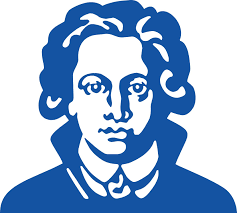
\includegraphics{logo.png}}
}
\author{Jan van Dick}
\date{\today}

\begin{document}

\maketitle
\frontmatter


\chapter*{Abstrakt}
Friedrich Nietzsches These vom Tode Gottes, dass \glqq wir\grqq{} ihn getötet haben, ist mehr als bloße Negativität. 
Müsste der Mensch nicht selbst Gott werden, um ihn getötet zu haben?.\footfullcite[Vgl.][481]{nietzsche_morgenrote_1999} 
Und der Mensch ist Gott dadurch geworden, dass er ihn \textit{geschaffen} hat, dadurch nur konnte er ihn töten. 
In dem Tod Gottes, liegt, dass Gott selbst vom Menschen gesetzt, dass er Schein ist, der sich gegen ihn verselbstständigte.
Gott ist somit geistiges Produkt des Menschen, in dem der Geist selbst wieder zur Natur sich verkehrte.
Der Tod Gottes ist die Befreiung daraus.
Der \glqq Tolle Mensch\grqq{} erklärt aber zugleich, dass nur die wenigsten von dieser Tat wissen. 
Für die Einen ist der Tod Gottes, eine untergegangene Sonne, die Befreiung also wieder eine In-Natur-Verkehrtheit.
Nur für uns \glqq geborene Räthselrather\grqq, die den Tod Gottes im vollen Umfang begreifen, ist er ein \glqq neues offenes Meer\grqq\footATCite[][573]{nietzsche_morgenrote_1999}.
Ist nun der Tod Gottes, die Befreiung aus der von ihm gesetzten Natur, das unbekannte, neue, offene, noch nie so offen gewesene Meer, oder ist er der Beginn des Wieder-in-Natur-Verkehrt-Seins, wie Christoph Menke es in der Analyse Hegels Begriffs der zweiten Natur beschreibt?\footfullcite[Vgl.][144]{menke_autonomie_2018}\\
Befreiung steht also zwischen Kritik (wieder-in-Natur-Verkehrtheit) und Affirmation (Einheit von Setzen und Sein).
Während Menke (und Hegel) Befreiung aus der zweiten Natur, nicht ohne eine neu hervorgebrachte zweite Natur, in welcher der Geist wieder in Natur verfällt lesen, erörterte ich die Frage, ob es in dem Motiv des \glqq neuen offenen Meeres\grqq{} und der \glqq geborenen Räthselrather\grqq{} bei Nietzsche, eine Befreiung aus der fortwährenden In-Natur-Verkehrtheit geben kann.
Es ist die Frage nach einer dritten Befreiung neben der Befreiung aus der 1. und der 2. Natur. 
Die Antwort dazu wird sich in der Arbeit als Ergebnis des Unterschiedes der \glqq Erkennenden\grqq{} bei Nietzsche geben:
Zwar kann Befreiung aus der Natur nicht ohne Setzen einer zweiten Natur geschehen, aber die Befreiung, die sich in dem Bewusstsein ihrer eigenen Kritik vollzieht, ist zugleich über ihrer eigene Befreiung hinaus.
Die dritte Befreiung ist damit allerdings keine Befreiung aus der Befreiung.
Befreiung bleibt notwendig: der Mensch kann Freiheit nicht \textit{haben}, er muss sie immer wieder selbst hervorbringen.


\tableofcontents

\mainmatter

\chapter{Einleitung}
So, wie Friedrich Nietzsche in dem Aphorismus vom \glqq Tollen Menschen\grqq{} in \textit{Die fröhliche Wissenschaft} die These vom Tode Gottes entfaltet, enthält sie weit mehr als die bloße Negation Gottes;
in ihr steckt eine dialektische Konzeption der Begriffe (zweite) Natur und Befreiung.\footfullcite[Vgl.][481]{nietzsche_morgenrote_1999}
Diese beiden Begriffe möchte ich aus der sprachgewaltigen und metaphergeladenen Sicht Nietzsches, sowie der von Christoph Menke rekonstruierten Perspektive Hegels untersuchen.
Beide Begriffe entfalten sich in ihrem Doppelcharakter: zweite Natur - Kritik und Affirmation, Befreiung - Macht und Ohnmacht des Geistes.
In der zweiten Natur schlägt Setzen in Sein um; hierin liegt zum Einen die Verwirklichung des Geistes (Affirmation), zum Anderen, die In-Natur-Verkehrtheit, der Tod des Geistes im Geist (Kritik).\footfullcite[Vgl.][145]{menke_autonomie_2018}
Ebenso verhält es sich mit dem Begriff der Befreiung: 
Sie ist 1. die \textit{Macht} des Geistes neues Hervorzubringen und die Notwendigkeit des Bestehenden zu durchbrechen, 
2. aber die \textit{Ohnmacht} des Geistes, da die Befreiung nie abgeschlossen ist; die Macht der Befreiung ist die Schaffung einer \glqq neuen\grqq{} zweiten Natur, aus der der Geist sich befreite und nun erneut befreien muss.\footATCite[Vgl.][80]{menke_autonomie_2018}\\
Doch während in Hegels Deutung der Geist in der Befreiung aus der zweiten Natur, auf Grund der Endlichkeit des menschlichen Geistes, wieder in Natur verfällt, scheint bei Nietzsche in der Metapher des neuen, offenen Meeres, die Perspektive die ewige Wiederholung der In-Natur-Verkehrtheit zu überwinden, gegeben zu sein.
Zugleich betonen sowohl Hegel, als auch Nietzsche Freiheit als nicht-gegeben: 
Freiheit wird bei beiden so gedacht, dass man sie \glqq nicht nur hat, sondern auch beständig  noch erwirbt und erwerben muss\grqq\footATCite[][637]{nietzsche_morgenrote_1999}. 
Freiheit ist die Befreiung aus der jeweiligen Unfreiheit.\footfullcite[Vgl][227]{adorno_negative_dialektik_2003} \\
Die Dialektik zwischen Freiheit und Notwendigkeit, Geist und Mechanismus, Endlichkeit und Unendlichkeit des Geistes, ist demnach Grundlage meiner Arbeit. 
Die Leitfrage der Arbeit also: \textit{gibt es in Nietzsches Philosophie eine Möglichkeit der Überwindung der Notwendigkeit-in-Natur-Verkehrtheit des Geistes?}\\
Aus der Position des oben erwähnten \glqq Tollen Menschen\grqq{} liegt es nahe, diese Möglichkeit in dem \textit{Vollzug} der Befreiung zu denken. 
Genauer: in einer Form des Bewusstseins in der Tätigkeit der Befreiung; 
eine Befreiung, die sich im Bewusstsein ihrer eigenen Kritik vollzieht.
Zu Fragen ist, ob dieses Bewusst-Werden eine Arbeit des einzelnen Individuums ist, oder ob es aus der Struktur des Allgemeinen, aus der zweiten Natur selbst, hervorgehen kann.\\

Der Begriff der zweiten Natur soll zunächst aus der Position Hegels heraus entwickelt werden, als eine Kritik an Kants Begriff der Autonomie. 
Darin ergibt sich, wie oben angegeben, die Grenze des von Menke erarbeiteten Begriffs der Befreiung:
Macht und Ohnmacht der Befreiung: Freiheit und Unfreiheit bleiben untrennbar miteinander verbunden.
Durch die Hinzunahme Nietzsches, soll versucht werden über diese Grenze hinauszugehen.
Dazu soll zunächst der Begriff der zweiten Natur aus der Perspektive Hegels erläutert werden. 
In einem \hyperref[abschnitt_1]{ersten Schritt} soll demnach der Hegelsche Begriff der zweiten Natur anhand von folgendem Zitat Menkes rekonstruiert werden:
\begin{itemize}
    \item[] Die Gewohnheit als zweite Natur [ist] geistig oder frei [...], insofern sie ein Ausdruck des Wollens (oder ein Setzen) ist, und [...] mechanisch oder unfrei [...], weil sie, einmal gesetzt, selbstständig und unbewusst wirkend ist.\footATCite[][145]{menke_autonomie_2018}
\end{itemize}
Die Struktur des ersten Teils ergibt sich aus den zu klärenden Begriffen. 
Zuerst soll der Begriff der Gewohnheit aus der Sittlichkeit, als Schritt über den \glqq bloß moralischen Standpunkt[]\grqq\footfullcite[][§ 135, S.139]{hegel_grundlinien_2017} hinaus, erläutert werden (a). 
Daraus ergibt sich der Begriff des \glqq geistigen Mechanismus\grqq, in welchem die Gewohnheit sich als \glqq geistig oder frei\grqq{} und \glqq mechanisch oder unfrei\grqq{} ergibt.\footATCite[][145]{menke_autonomie_2018} (b).
Schließlich soll der Begriff der zweiten Natur aus Hegels Perspektive, seinen Abschluss finden in der Dialektik zwischen endlichem und unendlichem Geist und dem Doppelcharakter der zweiten Natur als Kritik und Affirmation (c).\\
In einem \hyperref[abschnitt_2]{zweiten Schritt} soll gezeigt werden, dass bei Nietzsche ein ähnlicher Begriff der zweiten Natur aufgezeigt werden kann.\footnote{Ich halte diesen Schritt unter anderem des deshalb für sinnvoll, weil er rechtfertigt, warum ich meine mit Nietzsche überhaupt über Menkes Begriff der Befreiung hinausgehen zu können.}
Dabei soll bereits auf die Beantwortung der Leitfrage vorbereitet, aber diese noch nicht beantwortet werden.
Zunächst soll der Begriff der zweiten Natur anhand von Nietzsches Begriff des \textit{Scheins} erläutert werden (a).
Die Befreiung aus dem (sog.) Schein wird darauffolgend in der Unterscheidung des Schauspielers und der Rolle aufgegriffen (b). 
Abschließend sollen beide Begriffe nochmals in dem Absatz über den tollen Menschen analysiert und zusammengebracht werden (c).
In der Darlegung von Nietzsches Position, wird der Begriff des Bewusstseins des Scheins bereits eine wichtige Rolle einnehmen und dient der späteren Beantwortung der Leitfrage.\\
Zunächst soll im \hyperref[abschnitt_3]{dritten Schritt} noch der Begriff der Befreiung aus der zweiten Natur erläutert werden, da dieser im Vergleich zur Befreiung aus der ersten Natur bei Hegel und Menke und letztendlich auch bei Nietzsche uneindeutig bleibt.
Wie Befreiung aus der zweiten Natur überhaupt möglich ist und wie diese sich konkret vollzieht, ist notwendig, um zu diskutieren, wie über diese hinausgegangen werden kann.\\
Im vierten und \hyperref[abschnitt_4]{letzten Schritt} soll es abschließend zu einer Diskussion und Beantwortung der Leitfrage kommen. 


\chapter{Hauptteil}
\section{Zweite Natur bei Hegel}\label{abschnitt_1}
\subsection{(a) Autonomie und Sittlichkeit}
\subsection{(b) Dialektik von Geist und Mechanismus}
\subsection{(c) Dialektik von Kritik und Affirmation}
\section{Zweite Natur bei Nietzsche}\label{abschnitt_2}
\subsection{(a) Was bedeutet Schein?}
\subsection{(b) Der Schauspieler und die Rolle}
\subsection{(c) Gott ist tot!}
\section{Was heißt Befreiung aus der zweiten Natur}\label{abschnitt_3}
\section{Das offene Meer?}\label{abschnitt_4}

\chapter{Fazit}

\backmatter

\printbibliography
 
\end{document}
